\documentclass[article,english]{stucosrec}

% Example of defining a new command
\newcommand{\latex}{\LaTeX\xspace}
\newcommand{\bibtex}{Bib\TeX\xspace}
\newcommand{\stucosrec}{StuCoSReC\xspace}
\newcommand{\latexe}{\LaTeX$2_\epsilon$\xspace}

\title{\stucosrec AUTHORS GUIDE FOR CONTRIBUTION}
\author{
	Klemen Berkovi\v{c} \\
	Faculty of Electrical \\Engineering and Computer Science,\\
	University of Maribor,\\
	Koro\v{s}ka cesta 46, 2000 Maribor, Slovenia \\
	\texttt{klemen.berkovic1@um.si}
	\And
	Iztok Fister\\
	Faculty of Electrical \\Engineering and Computer Science,\\
	University of Maribor,\\
	Koro\v{s}ka cesta 46, 2000 Maribor, Slovenia \\
	\texttt{iztok.fister@um.si}
	\AND
	Janez Brest\\
	Faculty of Electrical \\Engineering and Computer Science,\\
	University of Maribor,\\
	Koro\v{s}ka cesta 46, 2000 Maribor, Slovenia \\
	\texttt{janez.brest@um.si}
}

% images directory
\imagespath{ {./images/} }

\begin{document}
    \maketitle
    
    \begin{abstract}
        A single paragraph of about 200 words maximum.
        For research articles, abstracts should give a pertinent overview of the work.
        We strongly encourage authors to use the following style of structured abstracts, but without headings: 
        \begin{inparaenum}
            \item Background: place the question addressed in a broad context and highlight the purpose of the study;
            \item Methods: describe briefly the main methods or treatments applied;
            \item Results: summarize the article’s main findings;
            \item Conclusion: indicate the main conclusions or interpretations.
        \end{inparaenum}
        The abstract should be an objective representation of the article, it must not contain results which are not presented and substantiated in the main text and should not exaggerate the main conclusions.
    \end{abstract}
    
    \keywords{\stucosrec Proceedings \and Author guide \and \latex}
    
    \section{Introduction}
    
    The introduction should briefly place the study in a broad context and highlight why it is important. 
    It should define the purpose of the work and its significance.
    The current state of the research field should be reviewed carefully and key publications cited.
    Please highlight controversial and diverging hypotheses when necessary.
    Finally, briefly mention the main aim of the work and highlight the principal conclusions.
    As far as possible, please keep the introduction comprehensible to scientists outside your particular field of research.
    Citing journal papers~\cite{bowman:reasoning, braams:babel}.
    Now citing a book reference~\cite{Lamport:LaTeX, salas:calculus} and booklets~\cite{CitekeyBooklet} or other references types~\cite{vrbancic2019transfer, clark:pct, CitekeyMisc}.
    
    \section{Materials and Methods}
    
    Materials and Methods should be described with sufficient details to allow others to replicate and build on published results.
    Please note that publication of your manuscript implicates that you must make all materials, data, computer code, and protocols associated with the publication available to readers.
    Please disclose at the submission stage any restrictions on the availability of materials or information.
    New methods and protocols should be described in detail while well-established methods can be briefly described and appropriately cited.
    
    Research manuscripts reporting large datasets that are deposited in a publicly avail-able database should specify where the data have been deposited and provide the relevant accession numbers.
    If the accession numbers have not yet been obtained at the time of submission, please state that they will be provided during review.
    They must be provided prior to publication.
    
    Interventionary studies involving animals or humans, and other studies require ethical approval must list the authority that provided approval and the corresponding ethical approval code.
    
    \section{Results}
    
    This section may be divided by subheadings.
    It should provide a concise and precise description of the experimental results, their interpretation as well as the experimental conclusions that can be drawn.
    
    \subsection{Subsection}
    
    \subsubsection{Subsubsection}
    
    \begin{itemize}
		\item First item,
		\item Second item and
		\item Third item.
	\end{itemize}
	
	\begin{enumerate}
	    \item First point,
	    \item Second point,
	    \item $\cdots$
	\end{enumerate}
    
    \subsection{Figures and Tables}
    
    Sample of figures in Figure~\ref{fig:circles}, Figure~\ref{fig:star} and Figure~\ref{fig:spin}.
    
    \begin{figure}
		\centering
		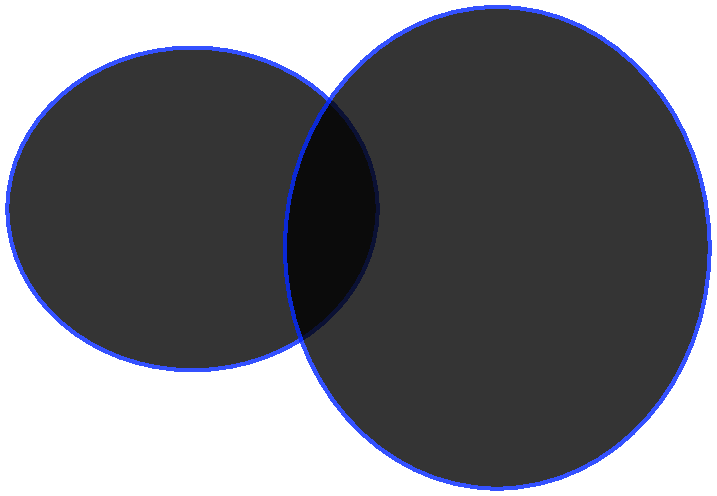
\includegraphics[scale=0.5]{circles.pdf}
		\caption{A sample circles graphic (\texttt{.pdf} format).}
		\label{fig:circles}
	\end{figure}
	
	\begin{figure}
		\centering
		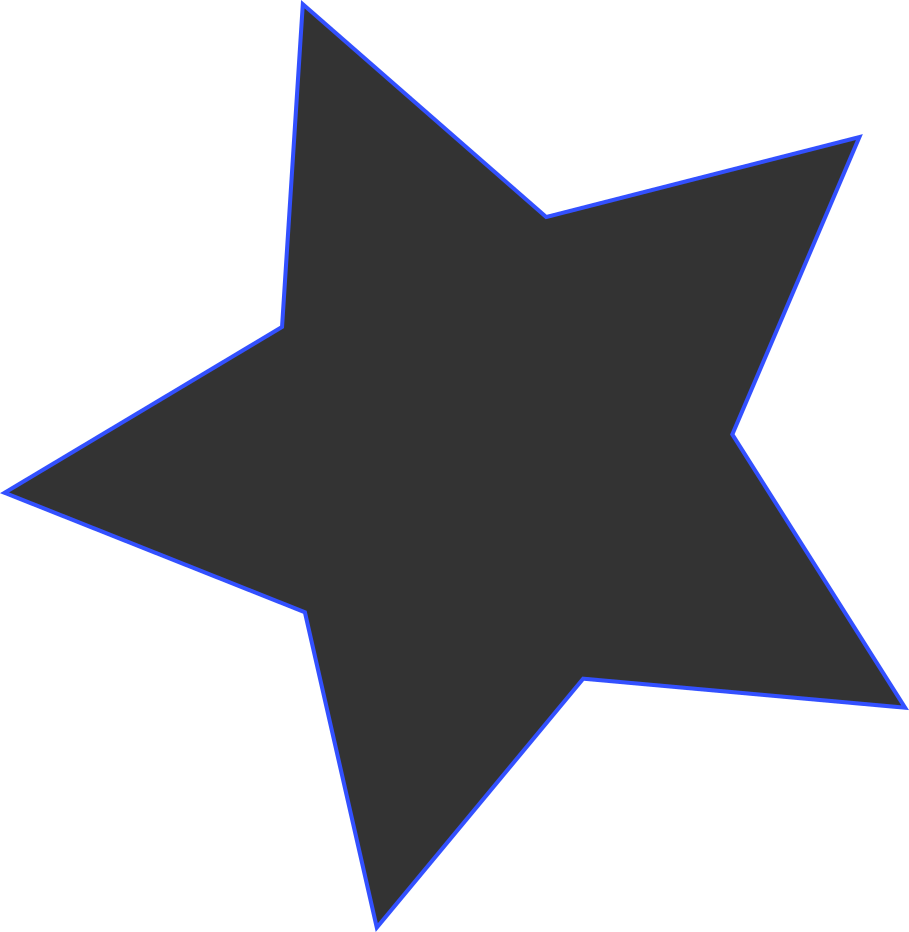
\includegraphics[scale=0.5]{star.png}
		\caption{A sample star graphic (\texttt{.png} format).}
		\label{fig:star}
	\end{figure}
	
	\begin{figure*}
		\centering
		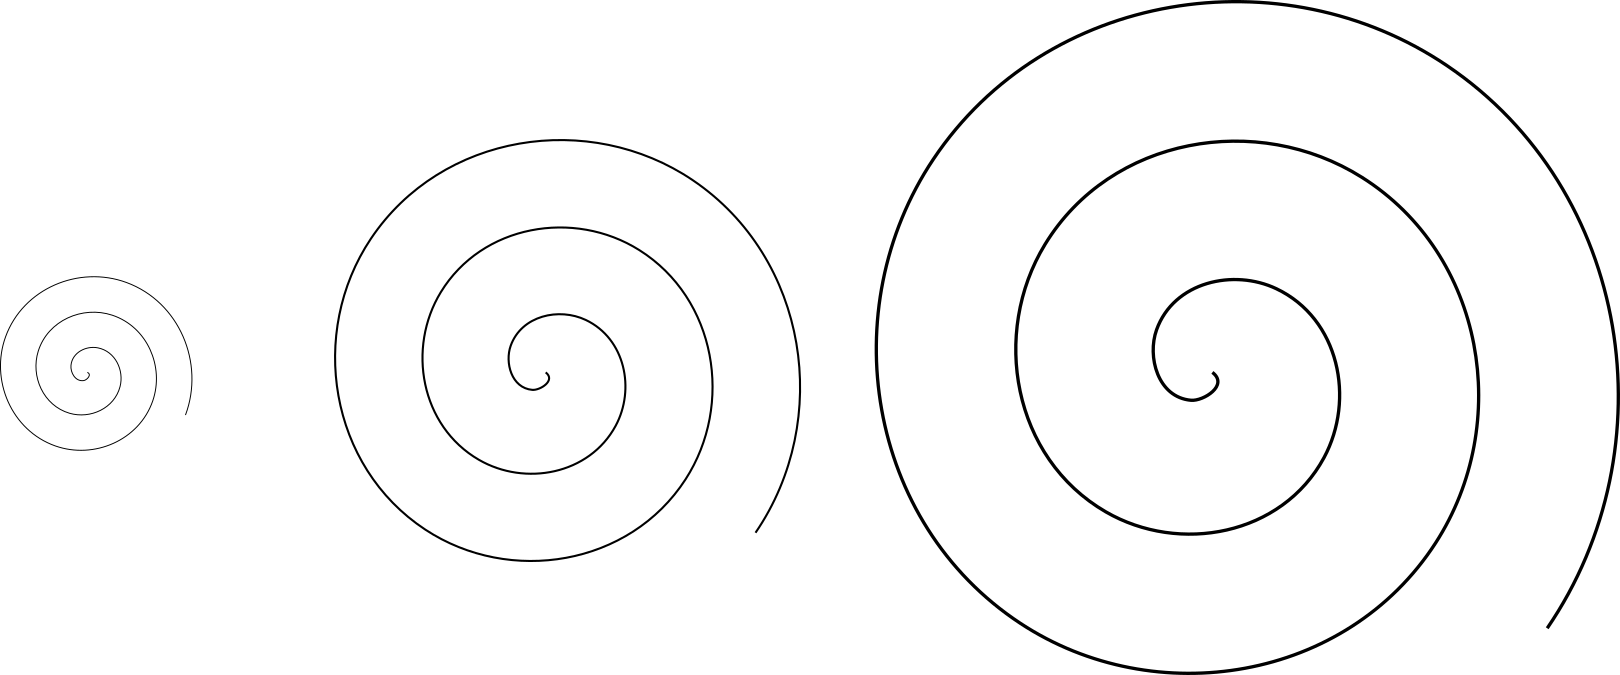
\includegraphics[scale=0.8]{spin.png}
		\caption{A sample spin graphic with a span.}
		\label{fig:spin}
	\end{figure*}
	
	Sample of tables in Table~\ref{tab:table1} and Table~\ref{tab:table2}.
	
	\begin{table}
		\centering
		\caption{Frequency of Special Characters.}
		\label{tab:table1}
		\begin{tabular}{|c|c|l|} \hline
			Non-English or Math&Frequency&Comments\\ \hline
			\O & 1 in 1,000& Swedish names\\ \hline
			$\pi$ & 1 in 5& In math\\ \hline
			\$ & 4 in 5 & In business\\ \hline
			$\Psi^2_1$ & 1 in 40,000& Unexplained \\ \hline
		\end{tabular}
	\end{table}
	
	\begin{table*}
		\centering
		\caption{Some Typical Commands.}
		\label{tab:table2}
		\begin{tabular}{|c|c|l|} \hline
			Command&A Number&Comments\\ \hline
			\texttt{{\char'134}imagespath} & 200 & For directory of included images \\ \hline
			\texttt{{\char'134}table} & 300 & For tables\\ \hline
			\texttt{{\char'134}table*} & 400& For wider tables\\ \hline
		\end{tabular}
	\end{table*}
    
    \subsection{Formatting of Mathematical Components}
    
    When $a \ne 0$, there are two solutions to $ax^2 + bx + c = 0$ and they are $$x_{1, 2} = \frac{-b \pm \sqrt{b^2-4ac}}{2a}.$$
    
    \begin{displaymath}\sum_{i=0}^{\infty} x + 1\end{displaymath}
    
    \begin{equation}
		\begin{aligned} 
			\mathrm{nr}(G_i,r) & = \label{equ:yannibel}
			\begin{cases}
				1  & \text{$r$ is played by one member of $G_i$}\\
				-2 & \text{$r$ is not played in $G_i$} \\
				-p & \text{$r$ is played by $p$ members in $G_i$}\\
			\end{cases}
		\end{aligned}
	\end{equation}
	
	\begin{equation}
		\begin{aligned}
			O_{\max}& = w_1 \sum_{a=1}^{m} \sum_{b=a+1}^{n} (-\lvert\text{CPT}_a 
			-\text{CPT}_b\rvert)\\ 
			&\quad + w_2 \sum_{j=1}^{m} (\text{DIF}_j) + w_3 \sum_{j=1}^{m} 
			(\text{INT}_j/\sum_{x=1}^{n} x_{ij})
		\end{aligned}
		\label{equ:ho}
	\end{equation}
    
    \subsection{Algorithms}
    
    \begin{algorithm}
		\SetAlgoLined
		\KwData{this text}
		\KwResult{how to write algorithm with \latexe}
		initialization\;
		\tcc{this is a comment to tell you that we will now really start code}
		\While{not at end of this document}{\label{algo:sample:while}
			read current\;
			\eIf{understand}{
				go to next section\;
				current section becomes this one\;
			}{
				go back to the beginning of current section\;
			}
		}
		\caption{How to write algorithms.}
		\label{algo:sample}
	\end{algorithm}
    
    \section{Discussion}
    
    Authors should discuss the results and how they can be interpreted from the perspective of previous studies and of the working hypotheses.
    The findings and their implications should be discussed in the broadest context possible.
    Future research directions may also be highlighted.
    
    \section{Conclusions}
    
    This section is not mandatory, but can be added to the manuscript if the discussion is unusually long or complex.
    
    \section{Patents}
    
    This section is not mandatory, but may be added if there are patents resulting from the work reported in this manuscript.
    
    \begin{acknowledgment}
		This section is optional; it is a location for you to acknowledge grants, funding, editing assistance and what have you.
		In the present case, for example, the authors would like to thank Klemen Berkovič for his help in codifying this \textit{Author's Guide}, the \texttt{.cls} and \texttt{.tex} files that is describes. Authors would like to thank Iztok Fister Jr. for his contribution to \textit{Author's Guide} and \texttt{.tex} files.
	\end{acknowledgment}
    
    \bibliography{references}
    
\end{document}